\documentclass[aspectratio=169,11pt]{ctexbeamer}

\usepackage{graphicx}
\usepackage{booktabs}
\usepackage{tabularx}
\usepackage{array}
\usepackage{xcolor}
\usepackage{hyperref}

\usetheme{Boadilla}
\usecolortheme{default}
\setbeamertemplate{navigation symbols}{}
\setbeamertemplate{footline}[frame number]
\setbeamercolor{title}{fg=white,bg=blue!55!black}
\setbeamercolor{frametitle}{fg=blue!35!black}
\setbeamercolor{block title}{fg=white,bg=blue!55!black}
\setbeamercolor{block body}{bg=blue!4!white}
\setbeamercolor{alerted text}{fg=red!65!black}

\graphicspath{{figures/}}
\hypersetup{colorlinks=true,linkcolor=blue!45!black,urlcolor=blue!45!black}

\newcommand{\ok}{\textcolor{green!45!black}{已完成}}
\newcommand{\risk}{\textcolor{orange!80!black}{待完善}}
\newcommand{\code}[1]{\texttt{\small #1}}

\title[Proj57 初赛演示]{Proj57 初赛演示：ACT 模型在 RK3588 上的 RKNN 推理闭环}
\subtitle{面向具身智能的国产操作系统 ACT 模型适配与实时推理优化}
\author{李捷铭（队长，清华大学）\quad 朱屹帆\quad 杨若朝}
\institute{OS 功能挑战赛道 Proj57}
\date{2026 年 6 月 30 日}

\begin{document}

\begin{frame}
  \titlepage
  \vspace{-0.6em}
  \begin{center}
    \small 核心结论：ONNX 到 RKNN 转换已完成，Orange Pi RK3588 板端 C++ RKNN runtime 已跑出两个代表样例。
  \end{center}
\end{frame}

\begin{frame}{本次展示要证明什么}
  \begin{block}{赛题目标}
    使用统一 ACT 模型，在 StarryOS/QEMU 与嵌入式平台上完成推理部署，输出动作预测结果。
  \end{block}
  \begin{itemize}
    \item 任务三：QEMU/StarryOS CPU 路线，是初赛保底链路。
    \item 任务二：Orange Pi RK3588/NPU 路线，是当前硬件适配主线。
    \item 本次展示重点：证明任务二的最小推理闭环已经真实跑通，而不是只停留在方案设计。
  \end{itemize}
\end{frame}

\begin{frame}{我们实际完成的链路}
  \begin{columns}[T,onlytextwidth]
    \begin{column}{0.48\textwidth}
      \begin{block}{模型链路}
        \begin{itemize}
          \item PyTorch checkpoint：\code{model.pt}
          \item 导出 ONNX：\code{act.onnx}
          \item 转换 RKNN：\code{act\_rk3588\_fp.rknn}
          \item 板端 C++ 调用：\code{librknnrt.so}
        \end{itemize}
      \end{block}
    \end{column}
    \begin{column}{0.48\textwidth}
      \begin{block}{动作判断}
        \begin{itemize}
          \item 输入：图像、机器人状态、latent 向量
          \item 输出：未来 8 步 action
          \item 第一维：\code{left\_vel}
          \item 第二维：\code{right\_vel}
          \item 判断：左轮速度小于右轮速度时为 LEFT
        \end{itemize}
      \end{block}
    \end{column}
  \end{columns}
\end{frame}

\begin{frame}{板端证据 1：Orange Pi 5 Plus 实物与系统}
  \begin{columns}[T,onlytextwidth]
    \begin{column}{0.42\textwidth}
      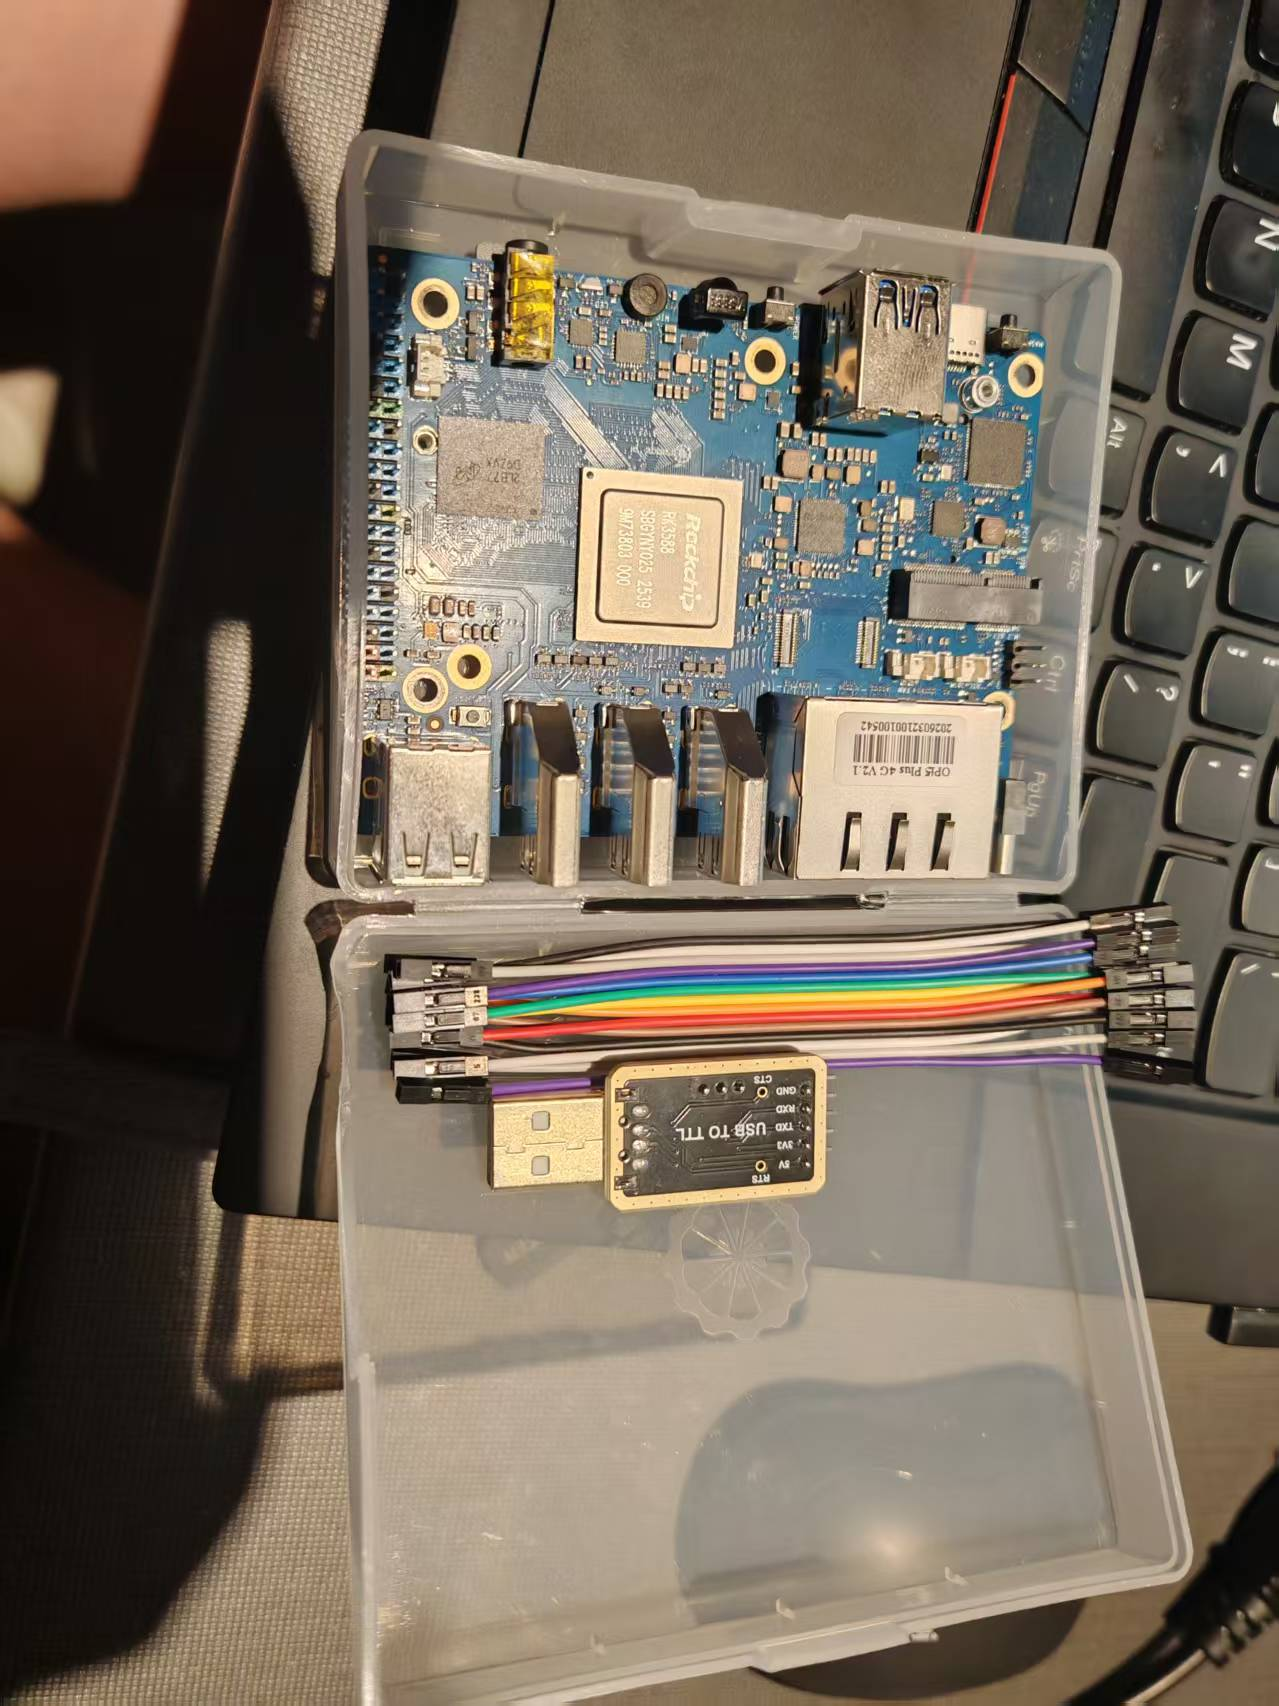
\includegraphics[width=\linewidth,height=0.70\textheight,keepaspectratio]{orange_pi_board_photo.png}
    \end{column}
    \begin{column}{0.56\textwidth}
      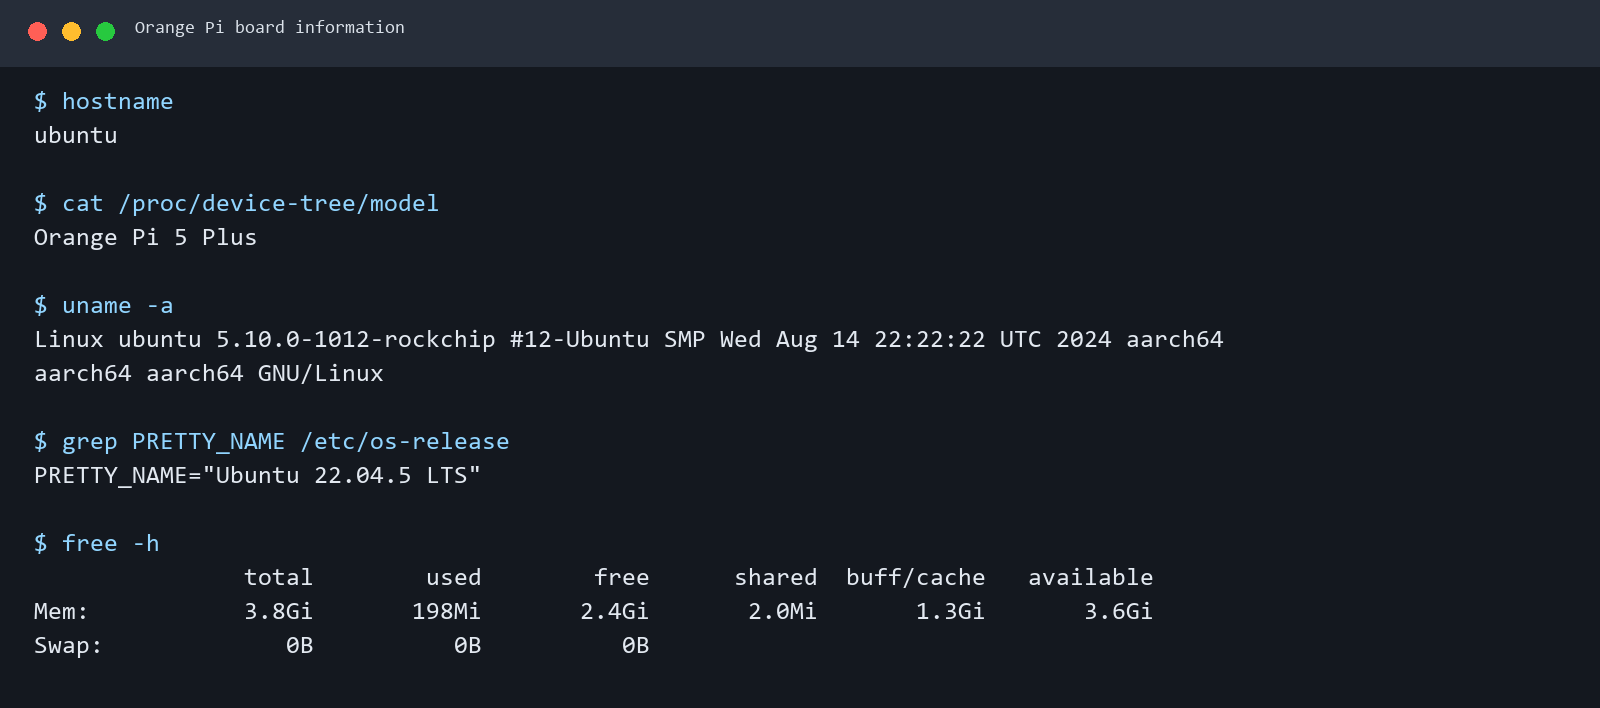
\includegraphics[width=\linewidth]{terminal_board_info.png}
    \end{column}
  \end{columns}
  \vspace{0.4em}
  \small 已确认板型为 Orange Pi 5 Plus，系统为 Ubuntu 22.04.5 LTS，架构为 aarch64，内存约 3.8 GiB。
\end{frame}

\begin{frame}{板端证据 2：NPU 节点与 RKNN Runtime}
  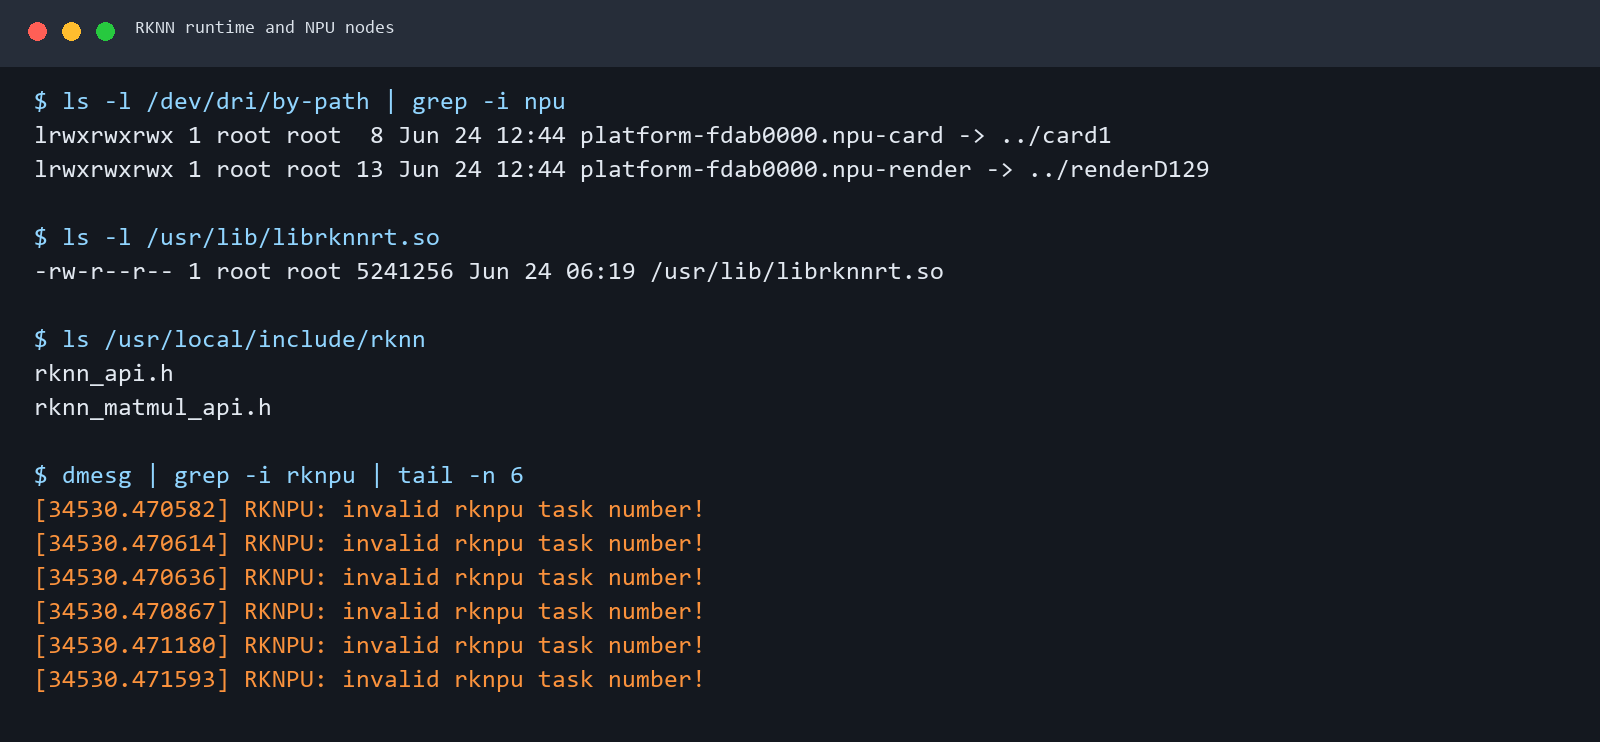
\includegraphics[width=\linewidth,height=0.72\textheight,keepaspectratio]{terminal_npu_runtime.png}
  \vspace{0.3em}
  \small 已确认 NPU DRM 节点、\code{/usr/lib/librknnrt.so} 和 RKNN 头文件存在。图中的 RKNPU warning 是后续需要处理的 runtime/driver 版本问题。
\end{frame}

\begin{frame}{ONNX 基线：先证明模型本身输出正确}
  \begin{block}{已复现的 ONNX Runtime 结果}
    \begin{itemize}
      \item \code{frame\_000000.jpg -> LEFT}，符合预期。
      \item \code{frame\_000227.jpg -> RIGHT}，符合预期。
      \item Windows 本机 ONNX Runtime CPU：两个样例平均约 25.91 到 26.78 ms。
      \item QEMU/StarryOS 既有报告结果：约 18.4 到 18.7 s，峰值内存约 454 MB。
    \end{itemize}
  \end{block}
  \begin{alertblock}{为什么先做 ONNX 基线}
    RKNN 输出不要求 bit-exact，但方向必须和基线一致。ONNX 基线是 RKNN 板端结果的正确性对照。
  \end{alertblock}
\end{frame}

\begin{frame}{RKNN 转换结果}
  \begin{columns}[T,onlytextwidth]
    \begin{column}{0.50\textwidth}
      \begin{block}{转换环境}
        \begin{itemize}
          \item WSL Ubuntu 24.04 / x86\_64
          \item \code{rknn-toolkit2 2.3.2}
          \item \code{torch 2.4.0+cpu}
          \item \code{onnx 1.16.2}
        \end{itemize}
      \end{block}
    \end{column}
    \begin{column}{0.46\textwidth}
      \begin{block}{模型大小}
        \begin{tabular}{lr}
          \toprule
          文件 & 大小 \\
          \midrule
          \code{model.pt} & 202,962,639 B \\
          \code{act.onnx} & 202,633,726 B \\
          \code{act\_rk3588\_fp.rknn} & 101,709,294 B \\
          \bottomrule
        \end{tabular}
      \end{block}
    \end{column}
  \end{columns}
  \vspace{0.4em}
  \small 转换脚本：\code{tools/convert\_act\_rknn.py}。板端运行程序：\code{tools/rknn\_runtime\_infer.cpp}。
\end{frame}

\begin{frame}{RKNN 板端运行结果：两个代表样例}
  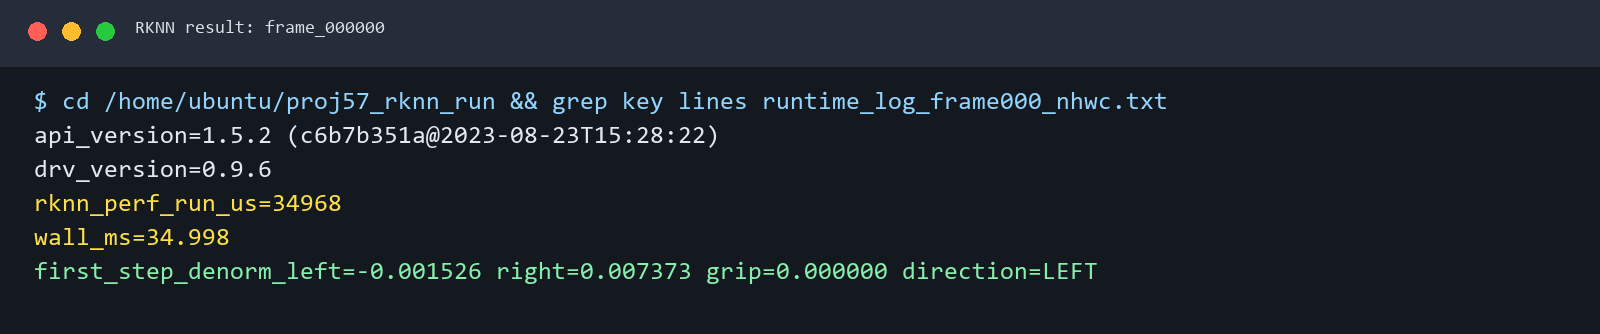
\includegraphics[width=\linewidth]{terminal_rknn_left.png}
  \vspace{0.4em}
  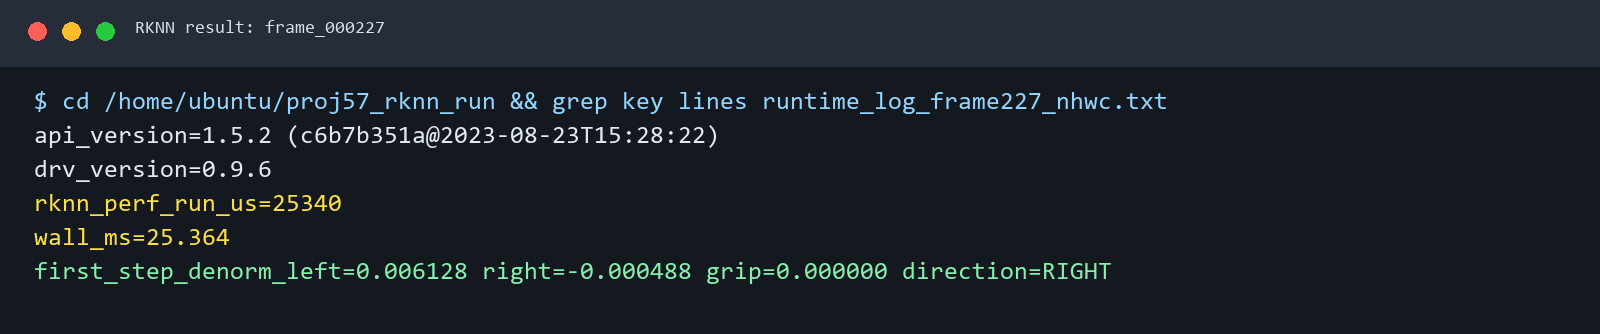
\includegraphics[width=\linewidth]{terminal_rknn_right.png}
  \vspace{0.4em}
  \small 结论：\code{frame\_000000 -> LEFT}，\code{frame\_000227 -> RIGHT}，方向与 ONNX 基线一致。
\end{frame}

\begin{frame}{性能与资源数据}
  \begin{table}
    \centering
    \small
    \begin{tabularx}{\linewidth}{l l l r r}
      \toprule
      平台 & 后端 & 状态 & 模型大小 & 推理耗时 \\
      \midrule
      QEMU/StarryOS & ONNX CPU & 已有报告 & 193.2 MB & 18.4--18.7 s \\
      Windows 本机 & ONNX CPU & 已复现 & 193.25 MB & 25.91--26.78 ms \\
      Orange Pi RK3588 & RKNN/NPU & 已跑通 & 97.0 MiB & 25.34--35.00 ms \\
      \bottomrule
    \end{tabularx}
  \end{table}
  \begin{itemize}
    \item RKNN runtime 返回的 \code{rknn\_perf\_run\_us} 分别为 34968 和 25340。
    \item 两个样例的 LEFT/RIGHT 方向与 ONNX 基线一致。
  \end{itemize}
\end{frame}

\begin{frame}{任务二现在到底完成到什么程度}
  \begin{columns}[T,onlytextwidth]
    \begin{column}{0.49\textwidth}
      \begin{block}{可以确认完成}
        \begin{itemize}
          \item \ok{} ONNX 模型导出
          \item \ok{} RKNN 模型转换
          \item \ok{} RK3588 板端 C++ runtime
          \item \ok{} 两个代表样例方向正确
          \item \ok{} 记录模型大小和推理耗时
        \end{itemize}
      \end{block}
    \end{column}
    \begin{column}{0.49\textwidth}
      \begin{alertblock}{仍需完善}
        \begin{itemize}
          \item \risk{} 当前输入是预处理后的 tensor bin
          \item \risk{} 还不是直接 JPEG 到推理输出
          \item \risk{} runtime 版本警告仍存在
          \item \risk{} 样例数量还需要扩展
        \end{itemize}
      \end{alertblock}
    \end{column}
  \end{columns}
  \vspace{0.3em}
  \small 稳妥表述：任务二 RK3588 平台 ACT 推理最小闭环已经跑通，后续进入工程化和稳定性优化。
\end{frame}

\begin{frame}{本次新增工程产物}
  \begin{itemize}
    \item 修复 ONNX 导出流程：避免下载 torchvision 预训练权重，自动创建 \code{build/} 目录。
    \item 新增 RKNN 转换脚本：\code{tools/convert\_act\_rknn.py}。
    \item 新增 RKNN 板端 C++ runtime：\code{tools/rknn\_runtime\_infer.cpp}。
    \item 采集板端证据：系统信息、NPU 节点、RKNN runtime、运行日志。
    \item 整理初审材料：技术文档、性能表、演示脚本、PDF 和本 PPT。
  \end{itemize}
  \vspace{0.3em}
  \small 板端同步目录：\code{/home/ubuntu/proj57\_initial\_review}。
\end{frame}

\begin{frame}{下一步计划}
  \begin{enumerate}
    \item 对齐 RKNN Toolkit2 与板端 runtime 版本，消除 \code{invalid run task counter} 警告。
    \item 把 C++ runtime 扩展为完整命令行工具，支持 JPEG 读取、resize、normalize、推理和后处理。
    \item 增加更多 LEFT/RIGHT 样例回归，记录精度漂移、耗时波动和内存占用。
    \item 面向任务一 SG2002 的 256 MB 内存约束，继续探索模型裁剪、量化和算子拆分。
  \end{enumerate}
\end{frame}

\begin{frame}{总结}
  \begin{block}{结论}
    我们已经完成从 \code{model.pt} 到 \code{act.onnx}，再到 \code{act\_rk3588\_fp.rknn}，最后在 Orange Pi RK3588 上通过 C++ RKNN runtime 输出动作方向的最小闭环。
  \end{block}
  \begin{itemize}
    \item 任务三结果提供保底正确性和对照。
    \item 任务二已经有真实板端运行日志和性能数据。
    \item 当前主要风险已经明确，后续工作路径清晰。
  \end{itemize}
\end{frame}

\end{document}
